\chapter{Tools And Scripts}


















\section{mmorpdnd.py}

\subsection{Purpose}

This script serves as the backbone for an array of automatic linking and logistical features within MMORPDND. These functionalities typically operate on all files, encompassing crucial elements such as the generation of directories, HTML index files at the directory summits, establishment of uniform headers and navigation for all HTML documents, seamless interlinking between files, refinement of both HTML and CSS code, and an array of additional capabilities. When ran, this script will perform the following actions in the following order:

\begin{enumerate}
	\item Create Directory Structures if not already existing.
	\item Create index files for each directory.
	\item Update each index file to link to all files and images within the directory.
	\item Update the headers of all html files to the template html header.
	\item Update the navigation of all html files to the template navigation html.
	\item Search and hyperlink all words found in all html files to the appropriate html file whose name matches the words found.
	\item Beautify the code.
\end{enumerate}







\subsection{Use}

The mmorpdnd.py script can be ran as a gui window or using the command line options. The two main features are `test' and `update'. The `test' feature will create fake files and then perform the update command on them. This is useful for testing if the features and newly added features are working properly. The `update' feature will perform a combination of tasks which updates all appropriate files to do the steps mentioned in the list above.

\subsubsection{GUI}

\begin{figure}[h]
	\centering
	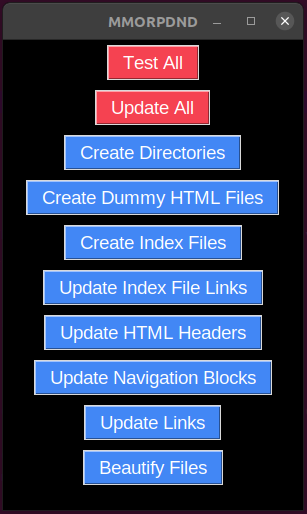
\includegraphics[width=0.5\textwidth]{images/mmorpdnd_gui.png}
	\caption{The MMORPDND Main GUI}
	\label{fig:mmorpdnd_gui}
\end{figure}

The GUI window is somewhat self explanatory. The two main features are represented by red buttons - the `test` and `update` features. There are also other buttons to simple perform and of the individual tasks using the appropriately associated button.

\subsubsection{Command Line}

The MMORPDND application supports some command line features.

\begin{lstlisting}
usage: mmorpdnd.py [-h] [-t] [-u]

MMORPDND Tools and apps.

optional arguments:
	-h, --help    show this help message and exit
	-t, --test    Runs the test-all feature then exit.
	-u, --update  Runs the update-all feature then exit.
\end{lstlisting}















\subsection{Programming Methods and Variables}

\begin{classbox}[class MMORPDND\_VARS]
"""
This is a class for storing variables used by MMORPDND* classes.
	
Methods:
	__init__(self)
	
Variables:
	# Define the directory structure
	self.directory_structure = { ... }
	
	# Define the number of HTML files to create in each subdirectory
	self.num_dummy_files_per_subdir = 3  # Stores all files created so far.
	self.all_index_files = []
	
	# Define the root directory
	self.root_dir = os.getcwd()
	self.script_dir = os.path.dirname(os.path.abspath(__file__))
	
	# Directories to exclude when processing.
	self.directories_to_exclude = ["templates", "css", ".git", ".idea", ".github", "scripts", "docs"]
	
	# Define the regular expression to match the header section
	self.header_regex = re.compile(r"<head>.*?</head>", re.DOTALL)
	
	# Define the regular expression to match the header section
	self.title_regex = re.compile(r"<title>.*?</title>", re.DOTALL)
	
	# Define the template file paths
	self.header_template_file = "templates/headerTemplate.html"
	self.nav_template_file = "templates/navTemplate.html"
	self.css_path = "css/mmorpdnd.css"
"""
\end{classbox}

\begin{codebox}[global\_vars = MMORPDND\_VARS()]
"""
Define a global variable containing the declared vars. Use this so they are all only defined once and can be updated/stored throughout the applications lifetime.
"""
\end{codebox}

\begin{codebox}[is\_image\_file(file\_name)]
"""
	Checks if a file name is an image file based on its extension.
	
Args:
	file_name (str): The name of the file to check.
	
Returns:
	bool: True if the file name has an image extension, False otherwise.
	
Example:
	>>> is_image_file('myphoto.jpg')
	True
	>>> is_image_file('document.pdf')
	False
"""
\end{codebox}


\begin{codebox}[get\_relative\_path(from\_file, to\_file)]
"""
Returns the relative path from one file to another.

Args:
	from_file (str): The path of the source file.
	to_file (str): The path of the target file.

Returns:
	str: The relative path from the source file to the target file.

Raises:
	None.

This method takes two file paths, `from_file` and `to_file`, and calculates the relative path from `from_file`
to `to_file`. The relative path represents the path that, when followed from `from_file`, leads to `to_file`.

Example:
	Assuming from_file = '/path/to/source/file.html' and to_file = '/path/to/target/image.jpg',
	the method will return '../../target/image.jpg' as the relative path.

Note: 
	The method uses the `os.path.relpath()` function to calculate the relative path.

Example usage:
	get_relative_path('/path/to/source/file.html', '/path/to/target/image.jpg')
	print(relative_path)  # Output: '../../target/image.jpg'
"""
\end{codebox}


\begin{codebox}[create\_dummy\_html\_files(directory=global\_vars.root\_dir)]
"""
Creates dummy HTML files in all directories and subdirectories for testing purposes.

Args:
	directory (str): The directory path to start creating dummy HTML files from. Defaults to global_vars.root_dir.

Returns:
	None.

Raises:
	None.

This method recursively walks through the directory structure, creates an index.html file in each directory,
and creates additional HTML files with random links in each subdirectory.

The method performs the following steps:
	1. Creates an index.html file in the specified directory with a basic HTML structure.
	2. Recursively walks through the directory structure using `os.walk`.
	3. For each subdirectory, excluding any directories listed in `global_vars.directories_to_exclude`:
		- Creates an index.html file in the subdirectory with a basic HTML structure.
		- Generates a specified number of dummy HTML files in the subdirectory, each containing a random link to another dummy file.
		- Prints a message indicating the successful creation of each HTML file.
	4. Creates additional dummy HTML files in the script directory (specified by the `directory` argument), each containing a random link to another dummy file.
	5. Prints a message indicating the successful creation of all HTML files.

Note: 
	The content of the generated HTML files consists of a basic HTML structure with a header and body.
Each dummy file includes a link to two randomly chosen dummy files, facilitating testing scenarios.

Example usage:
	create_dummy_html_files()
"""
\end{codebox}


\begin{codebox}[alphabetize\_links(list\_of\_links)]
"""
Alphabetizes the items in a list of links.

Args:
	list_of_links (str): A multiline string representing a list of links in the format
	"<li><a href="url">link_text</a></li>". Each link should be on a separate line.

Returns:
	str: A multiline string representing the alphabetized list of links.

Example:
	links = '''<li><a href="valen_shadowborn.html">valen_shadowborn</a></li>
	<li><a href="kaelar_stormcaller.html">kaelar_stormcaller</a></li>
	<li><a href="thorne_ironfist.html">thorne_ironfist</a></li>
	<li><a href="foobar.html">foobar</a></li>
	<li><a href="aria_thistlewood.html">aria_thistlewood</a></li>
	<li><a href="stoneshaper_golem.html">stoneshaper_golem</a></li>
	<li><a href="elara_nightshade.html">elara_nightshade</a></li>'''

	sorted_list = alphabetize_links(links)
	
	print(sorted_list)
"""
\end{codebox}


\begin{classbox}[class MMORPDND]
"""
A class for all the main MMORPDND features.

Methods:
	__init__(self)
	create_directories(self, path: str, structure: dict) -> None
	create_index_files(self, directory=global_vars.root_dir)
	move_dir_items_to_end(self, string)
	move_img_items_to_end(self, string)
	update_index_files(self)
	update_headers(self, directory=global_vars.root_dir)
	update_navigation(self, directory=global_vars.root_dir)
	beautify_files(self, directory=global_vars.root_dir)
	find_all_html_files(self, directory=global_vars.root_dir)
	update_html_links(self, directory=global_vars.root_dir)
"""
\end{classbox}


\begin{codebox}[MMORPDND.\_\_init\_\_(self)]
"""
Initialization method.
"""
\end{codebox}


\begin{codebox}[MMORPDND.create\_directories(self, path: str, structure: dict) -> None]
"""
Recursively creates directories in the given path according to the structure specified in the dictionary.

Args:
	path (str): The root path where directories will be created.
	structure (dict): A dictionary representing the structure of the directories to be created.

Returns:
	None
"""
\end{codebox}


\begin{codebox}[MMORPDND.create\_index\_files(self, directory=global\_vars.root\_dir)]
"""
Creates index files for all subdirectories within the specified directory.

Args:
	directory (str): The directory path to start creating index files from. Defaults to global_vars.root_dir.

Returns:
	None.

Raises:
	None.

This method traverses through all subdirectories and files starting from the specified directory and creates an
index file named "index.html" in each directory that doesn't already have one.

The method performs the following steps:
	1. Loop through all directories and files using `os.walk` starting from the specified directory.
	2. Check if an index file named "index.html" already exists in the current directory. If so, skip that directory.
	3. Check if the current directory matches any of the excluded directories defined in `global_vars.directories_to_exclude`.
	If so, skip that directory.
	4. Create an index.html file in the current directory.
	5. Write the HTML content to the index.html file, including the directory name in the title and header.
	6. Print a message indicating the creation of the index file.

Note: 
	The index.html file created contains a basic HTML structure with the title and header set to "Index of [directory_name]".

Example usage:
	create_index_files()
"""
\end{codebox}


\begin{codebox}[MMORPDND.move\_dir\_items\_to\_end(self, string)]
"""
Moves directory items (lines containing "/index.html") to the end of the input string.

This method takes a multi-line string as input and separates lines that contain "/index.html"
(directory items) from other lines (non-directory items). It then rearranges the lines by moving
the directory items to the end while maintaining the order of non-directory items.

Args:
	string (str): The input multi-line string to be processed.

Returns:
	str: A modified string with directory items moved to the end.

Example:
	input_string = "Line 1\n/index.html\nLine 2\nLine 3\n/index.html"
	result = move_dir_items_to_end(input_string)
	# result will be "Line 1\nLine 2\nLine 3\n/index.html\n/index.html"
"""
\end{codebox}


\begin{codebox}[MMORPDND.move\_img\_items\_to\_end(self, string)]
"""
Moves items containing "img/" to the end of the string while preserving their original order.

Args:
	string (str): A string containing items in the format '<li><a href="url">link_text</a></li>'.

Returns:
	str: A new string with items containing "img/" moved to the end while preserving their original order.

Example:
	>>> string = '''<li><a href="valen_shadowborn.html">valen_shadowborn</a></li>
	...            <li><a href="kaelar_stormcaller.html">kaelar_stormcaller</a></li>
	...            <li><a href="thorne_ironfist.html">thorne_ironfist</a></li>
	...            <li><a href="foobar.html">img/foobar</a></li>
	...            <li><a href="aria_thistlewood.html">img/aria_thistlewood</a></li>
	...            <li><a href="stoneshaper_golem.html">stoneshaper_golem</a></li>
	...            <li><a href="elara_nightshade.html">elara_nightshade</a></li>'''
	>>> new_string = move_img_items_to_end(string)
	>>> print(new_string)
	<li><a href="valen_shadowborn.html">valen_shadowborn</a></li>
	<li><a href="kaelar_stormcaller.html">kaelar_stormcaller</a></li>
	<li><a href="thorne_ironfist.html">thorne_ironfist</a></li>
	<li><a href="aria_thistlewood.html">img/aria_thistlewood</a></li>
	<li><a href="stoneshaper_golem.html">stoneshaper_golem</a></li>
	<li><a href="elara_nightshade.html">elara_nightshade</a></li>
	<li><a href="foobar.html">img/foobar</a></li>
"""
\end{codebox}


\begin{codebox}[MMORPDND.update\_index\_files(self)]
"""
Updates all index files in the directory and subdirectories to include links to other files in the same directory.

Returns:
	None.

Raises:
	None.

This method performs the following steps:
	1. Prints a message indicating that index files are being updated.
	2. Retrieves a list of all HTML index files in the current directory and subdirectories, excluding any directories listed in `global_vars.directories_to_exclude`.
	3. For each index file found:
		- Reads the file data.
		- Identifies the HTML files present in the same directory as the current index file.
		- If the index links div section does not exist in the file, it adds the div section just before the closing </body> tag.
		- Updates the index links by generating HTML code for each HTML file in the directory (excluding the index.html file) and appending it to the index links div.
		- Replaces the old index links section in the file with the updated index links div.
		- Writes the updated file data back to the file.
		- Prints a message indicating that the index file has been updated.
	4. Prints a message indicating that all index.html files have been updated.

Note: The method relies on regular expressions for searching and updating the index links section in each index file.

Example usage:
	update_index_files()
"""
\end{codebox}


\begin{codebox}[MMORPDND.update\_headers(self, directory=global\_vars.root\_dir)]
"""
Updates the headers of HTML files in the specified directory and its subdirectories to match a predefined template.

Args:
	directory (str): The directory path to update the HTML files in. Defaults to global_vars.root_dir.

Returns:
	None.

Raises:
	None.

This method performs the following steps:
	1. Loop through all HTML files in the specified directory and its subdirectories.
	2. For each HTML file found that does not contain "Template" in its filename:
		- Read the contents of the HTML file.
		- Check if the file is in the list of directories to exclude.
		- Read the contents of the header template file.
		- Replace the header section in the HTML file with the contents of the template.
		- Generate a title based on the filename and replace the title section in the HTML file.
		- Determine the relative path to the CSS file.
		- Calculate the number of subdirectories between the HTML file and the CSS file.
		- Create the correct link path for the CSS file.
		- Replace the placeholder in the HTML file with the link to the CSS file.
		- Overwrite the HTML file with the updated contents.
		- Print a progress update indicating the file that has been updated.
	3. Print a message indicating that the headers and CSS have been updated in all relevant HTML files.

Note: 
	The method relies on regular expressions for pattern matching and modification.

Example usage:
	update_headers()
"""
\end{codebox}


\begin{codebox}[MMORPDND.update\_navigation(self, directory=global\_vars.root\_dir)]
"""
Updates the navigation block of HTML files in the specified directory and its subdirectories to match a predefined template.

Args:
	directory (str): The directory path to update the HTML files in. Defaults to global_vars.root_dir.

Returns:
	None.

Raises:
	None.

This method performs the following steps:
	1. Loop through all HTML files in the specified directory and its subdirectories.
	2. For each HTML file found that does not contain "Template" in its filename:
		- Read the contents of the HTML file.
		- Check if the file is in the list of directories to exclude.
		- Print a progress message indicating the file being processed.
		- Read the contents of the navigation template file.
		- Find the navigation block in the original HTML file using a regular expression.
		- If a navigation block is found:
		- Replace the navigation block in the HTML file with the contents of the template.
		- Write the modified HTML back to the file.
		- Print a message indicating that the navigation block has been replaced.
		- If no navigation block is found:
		- Print a message indicating that the navigation block was not found.
		- Insert the navigation contents at the start of the body tag in the HTML file.
		- Overwrite the file with the updated contents.
		- Print a message indicating that the navigation contents have been inserted.

Note: 
	The method relies on regular expressions for pattern matching and modification.

Example usage:
	update_navigation()
"""
\end{codebox}


\begin{codebox}[MMORPDND.beautify\_files(self, directory=global\_vars.root\_dir)]
"""
Beautifies HTML and CSS files in the specified directory and its subdirectories.

Args:
	directory (str): The directory path to beautify the files in. Defaults to global_vars.root_dir.

Returns:
	None.

Raises:
	None.

This method performs the following steps:
	1. Modifies the directories_to_exclude list to include template and CSS files.
	2. Loops through all files and subdirectories in the specified directory.
	3. For each HTML or CSS file found (excluding those in the modified directories_to_exclude list):
		- Constructs the file path.
		- Checks if the file is an HTML or CSS file, and skips it if not.
		- Reads the contents of the file.
		- If the file is an HTML file:
		- Uses BeautifulSoup to parse the HTML and prettify it.
		- If the file is a CSS file:
		- Uses cssbeautifier to prettify the CSS code.
		- Writes the prettified code back to the file.
		- Prints a message indicating that the file has been prettified.

Note: 
	The method relies on BeautifulSoup for HTML parsing and prettifying, and cssbeautifier for CSS prettifying.

Example usage:
	navigator = Navigator()
	navigator.beautify_files()
"""
\end{codebox}


\begin{codebox}[MMORPDND.find\_all\_html\_files(self, directory=global\_vars.root\_dir)]
"""
Finds all HTML files (not index.html files) in a directory and its subdirectories.

Args:
	directory: The directory to search. Defaults to the current directory.
	
Returns: 
	A list of dictionaries containing the name (without extension), name (with extension), and full path
of each HTML file found.
"""
\end{codebox}


\begin{codebox}[MMORPDND.update\_html\_links(self, directory=global\_vars.root\_dir)]
"""
Update the links in the various HTML files to link to the appropriate file.

Args:
	directory (str): The directory to search for HTML files. Defaults to global_vars.root_dir.

Returns:
	None
"""
\end{codebox}

\begin{classbox}[class MMORPDND\_GUI]
"""
Class to store GUI functions and operations. The majority of the methods in this class simply connect the UI elements to the associated MMORPDND class methods.
	
Methods:
	__init__(self)
	run(self)
	test_all(self)
	update_all(self)
	create_directories(self)
	create_dummy_html_files(self)
	create_index_files(self)
	update_index_links(self)
	update_headers(self)
	update_navigation(self)
	beautify_files(self)
	update_html_links(self)
"""
\end{classbox}

\begin{codebox}[main()]
"""
Main method to start the gui and take optional arguments/parameters for running via command line.
"""
\end{codebox}













\section{templates/creator.py}



\subsection{Purpose}

The creator tool is a practical solution for converting basic template text files into functional HTML pages. It takes care of the technical aspects by automatically creating HTML files and filling in missing details, like character stats or other content. The tool understands the structure of your template files, recognizes placeholders, and replaces them with accurate data. Whether you're building character profiles, story summaries, or any content with consistent formatting, this tool ensures your HTML documents are correctly formatted and ready for use. It simplifies the process, letting you focus on content creation while it handles the conversion from templates to HTML.

\subsection{Use}

The creator tool is a powerful tool that contains many subtle features. It is important to understand these subtleties before using the tool and therefore I encourage the reader to read this enture section before use. 

\subsubsection{GUI}

\begin{figure}[h]
	\centering
	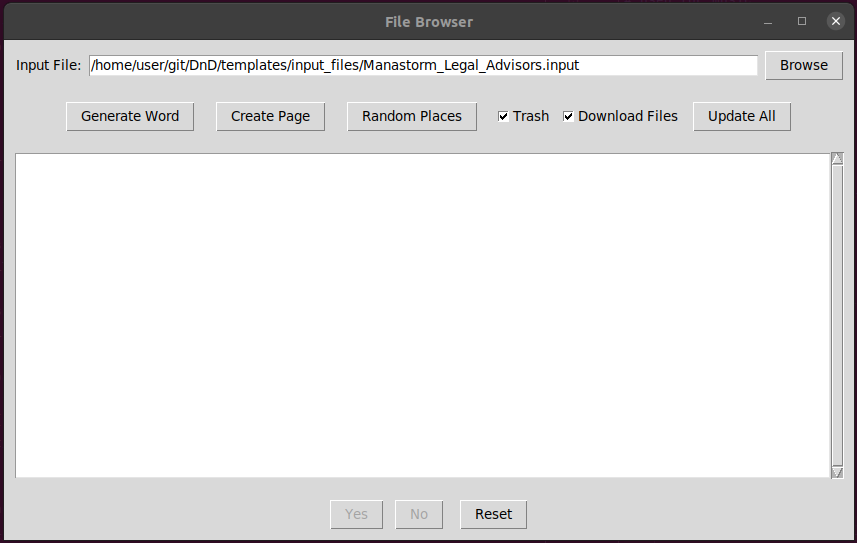
\includegraphics[width=0.9\textwidth]{images/creator_gui.png}
	\caption{The MMORPDND Main GUI}
	\label{fig:creator_gui}
\end{figure}

The main GUI of the creator tool has a few components. These include text boxes, buttons, and check boxes. 

The ``Input File" text box field is used to specify the input file that is to be processed by the tool. This file can be an `.input', `.char' or `.names' file. Ensure the file is in the proper format (see below sections) or unexpected behavior may occur. The `Browse' button is used to open a file explorer window for selecting a file and will automatically populate the ``Input File" text field when a file is selected. The large text box in the center of the GUI is where output generated from the tool as well as status messages are displayed.

The ``Generate Word" button is used for random word generation. This feature takes a list of words (whether names, places, or other) and generates a similar random word using the data in the input `.names' file. This is explained in more detail later in section \ref{section .names}. The ``Create Page'' button is used to generate an HTML file based on a `.input' or `.char' file and is explained in more details in the following sections. the ``Random Places'' file is used to generate place names based on an input `.names' file along with a `.list' file. These are explained mroe in later sections. The ``Yes", ``No", and ``Reset" buttons are used when user input is asked for. The ``Update All" button performs the same functions as the mmorpdnd.py update function (see the previous sections).

The ``Trash" checkbox will determine if processed files will be moved to the trash folder after processing and if duplicate files are to be deleted. Typically, the user will want this to be checked, but it is useful to leave unchecked for testing and if files will be processed multiple times. The ``Download Files" button determines if music files should be downloaded when `.input' files containing a dnd-music section are processed (this is explained mroe in later sections).

\subsubsection{Input Files (.input)}

The input files are essentially just text files with the file extension `.input'. The main feature of the creator.py tool is to read in these input files, parse them, and generate the appropriate html files from them. These input files must follow a strict formatting but offer a few various helpful features. Each line of the input file represents a 'section' of the html file that will be generated. Each line follows the following format:
\begin{lstlisting}
Heading Text[type]=Information text
\end{lstlisting}
The "Heading Text" is what will appear as the header for that html section. The "type" value is what determines the properties of this section and how it is interpreted by the creator tool. The "Information text" is the actual information for that section. The only exception to this rule is the first line which defines the "folder" that the html file generated from the input file will be placed into. This "folder" line is special in that it has no type and the creator tool will recognize the folder keyword and store this information separately. This folder line must be formatted as follows:
\begin{lstlisting}
folder=path/to/where/I/want/my/generated/file
\end{lstlisting}
The various types determine the formatting and decoding of the input file, and each type has small subtleties. The various types are
\begin{enumerate}
	\item dnd-image: This type is used to display an image or multiple images.
 	\item dnd-list: This is used to display a list of items.
 	\item dnd-info: This is used for general information and sections. It also supports listing information between paragraphs.
  	\item dnd-music: This is a section for storing various music for the regions.
\end{enumerate}

\subsubsection{dnd-image type}

The \textbf{dnd-image} type is used to display images specific to the file. The information text must contain three parameters separated by a semi-colon delimeter. These parameters are \textbf{img/image-name.jpg;image source;image caption}. The first parameter is simply the location of the image and the image name. These are typically placed in `templates/img'. The second is the source of the image, this is simply a string but is there to keep all images properly sourced. The third is a caption that will be displayed with an image. This caption is also a string and can be whatever the user desires. As an example, here's a proper dnd-image block:

\begin{lstlisting}
Coconatus Marmotta[dnd-image]=img/coconatus_marmotta.jpg;Created by Bing AI image creator;Coconatus Marmotta.
\end{lstlisting}

One unique feature of this is that if the image name does not exist (i.e. `img/coconatus\_marmotta.jpg'), the tool will append a ` (1)' to the name and search again (i.e. `img/coconatus\_marmotta (1).jpg'). If this new name is found, the tool will search for image names with the index incremented and include all such images (i.e. `img/coconatus\_marmotta (2).jpg', `img/coconatus\_marmotta (3).jpg', etc) in the output html block.  

\subsubsection{dnd-list type}

The \textbf{dnd-list} type is used to display a simple list of items. The information text must contain one or more parameters separated by a semi-colon delimeter. As an example, here's a proper dnd-list block:

\begin{lstlisting}
Landmarks and Other Features[dnd-list]=Talleril: A small island far off the coast of Alderpine.;Enthilma: A small island off the coast of Alderpine.;Lomelindei: The large world tree deep within Alderpine.
\end{lstlisting}

\subsubsection{dnd-info type}

SECTION IN PROGRESS!

\subsubsection{dnd-music type}

The \textbf{dnd-music} type is used to display a simple list of music items. The information text must contain one or more parameters separated by a semi-colon delimeter. Currently, this is primarily designed to work with youtube links. Given a simple youtube link, the code will find the name of the video and use that as the list information as well as keeping a link to the video itself. If the ``Download Links" checkbox in the GUI is enabled, the files will be downloaded as mp3 files and the folder next to the list item will be hyperlinked to the local file. These files will be located in a music folder. As an example, here's a proper dnd-music block (except with fake URL's):

\begin{lstlisting}
Music And Ambiance[dnd-music]=https://youtube_link_1;https://youtube_link_2;https://youtube_link_3
\end{lstlisting}




\subsubsection{Example Input File}

For example input files, you can look inside the templates/trash folder. This is where input files get placed after they are finished processing. The following is an example input file with an example of many different elements. The associated image files `foobar.jpg', `foobars (1).jpg' and `foobars (2).jpg' should be located in the templates/img folder for the below file to process correctly.

\begin{lstlisting}
folder=items

A Single Image[dnd-image]=img/foobar.jpg;Created by Someone;A foobar image.

Information Section[dnd-info]=Here is a paragraph of text.;Here is a second paragraph.

Information Section With Smaller Headers[dnd-info]=Here is a paragraph of text.;*Small Header* Here is a second paragraph.

A List Of Items[dnd-list]=item A; Item B; Item C; Item D

Multiple Images[dnd-image]=img/foobars.jpg;Created by Someone;Multiple foobar images.

Information Section with List[dnd-info]=Here is a paragraph of text followed by a list;-List_item_A;-List_item_B;-List_item_C;Followed by a paragraph.

Music And Ambiance[dnd-music]=https://youtube_link_1;https://youtube_link_2;https://youtube_link_3
\end{lstlisting}

The above file will create a file in the `items' folder found in `campaign/items'. The file will start with a header "A Single Image", where the foobar.jpg image is displayed. A caption of "A foobar image." will be under the image. Next will be a heading "Information Section" That has two paragraphs. Next a similar section with a header "Information Section With Smaller Headers", a paragraph, then a smaller header "Small Header", followed by another paragraph. Next, another heading "A List Of Items" with 4 items in the list. Following this, a "Multiple Images" heading with 2 images `foobars (1).jpg' and `foobars (2).jpg'\footnote{If an image is not found, it will automatically search for files with that image name with an appended (1), (2), (3),... If `(1)' is found, this image will be used and the number incrememted until no other images are found.} with a caption "Multiple foobar images." Next, another heading ``Information Section with List", with a paragraph, a list, and then another paragraph. Finally, a heading "Music And Ambiance" with links to three youtube videos. If the "download links" checkbox is enabled, these video's will be downloaded as mp3 files and the fodler icon will link to the local files.






\subsubsection{Character Files (.char)}

The character files are text files with the ".char" extension. These are a special type of input file that generates an html page specific for DnD character information. This was actually designed before the more general input file formatting outlined in the sections above and therefore lacks some of the versatility and extra features that can be included in the input files. Nevertheless, the character format creates an html page that should more than suffice for any npc characters and has many of its own unique features and capabilities. The .char file contains lines that define the various elements of a character. These lines to not currently support the types that are supported with the input files. Each line has a specific output format in the generated html file based on a template and the information itself. Some lines in the file are required while others are optional. The required lines must be present for the character file generated to be completed, while the optional lines will automatically be randomized and generated in the event that they are missing. Eahc line of the character file must be formatting in the following way:
\begin{lstlisting}
Keyword = Value
\end{lstlisting}
The "Keyword" is used by the creator tool to determine which type of information is being input, and the "Value" is the value of the information. For example "level = 3" would let the creator know that the character level is 3, and it will use that information appropriately.

Once the character file is appropriately filled out and created, it should be saved/placed in the templates/input\_files folder for processing by the creator tool just like the .input files. The creator tool will search the templates/img folder for any image references within the character files.






\subsubsection{Required Keywords}

The required keywords for a character file are the following:
\begin{enumerate}
	\item folder: This defines the folder that the output html character file will be placed. This should be a valid file path to a folder.
	\item name: This defines the name of the character.
	\item image: This is an image for the character. This should be just the image file name and extension (no path) and the image itself should be placed in the "templates/img" folder for automatic detection.
	\item class: This defines the DnD class. This must be a valid class from the following list:
		\begin{multicols}{3}
		    \begin{itemize}
		        \item barbarian
		        \item bard
		        \item cleric
		        \item druid
		        \item fighter
		        \item monk
		        \item paladin
		        \item ranger
		        \item rogue
		        \item sorcerer
		        \item warlock
		        \item wizard
		    \end{itemize}
		\end{multicols}
	\item abilities: The abilities of the character. This field is a list and should be entered using a comma (`,') as the delimeter.
	\item equipment: The equipment of the character. This field is a list and should be entered using a comma (`,') as the delimeter.
	\item proficiencies: These are the proficiencies of the character. This field is a list and should be entered using a comma (`,') as the delimeter. The proficiency bonus will automatically be calculated based on level and applied to proficiencies.
	\item information: General information and description of the character.
\end{enumerate}

The above list of keywords are all required and if they are missing or ill-formatted, unexpected behavior can occur.






\subsubsection{Optional Keywords}

The optional keywords for a character file are the following:
\begin{enumerate}
	\item level: This is the level of the character. If the level is not defined, it will default to 1. This must be an integer.
	\item hp: This will be generated automatically if not included based on the character class, level, and constitution\footnote{The constitution value is automatically generated based on the character class and level if not included.} value.
	\item ac: The Armor class value.
	\item size: The size of the character.
	\item type: The type of the character (creature, humanoid, animal, etc)
	\item alignment: The alignment of the character.
	\item speed: The speed of the character.
	\item resistances: The resistances the character has (if any).
	\item immunities: The immunities the character has (if any)
	\item senses: The senses. A ", Passive Perception: \#" will automatically be appended to this value based on a calculated passive perception.
	\item languages: Languages of the character.
	\item race: The race of the character.
	\item background: The background of the character.
	\item strength: This represents the character's physical strength and ability to exert force. This must be an integer.
	\item dexterity: This represents the character's agility, reflexes, and fine motor skills. This must be an integer.
	\item constitution: This measures the character's health, stamina, and resistance to illness and fatigue. This must be an integer.
	\item intelligence: This reflects the character's mental acuity, memory, and problem-solving skills. This must be an integer.
	\item wisdom: This represents the character's perception, intuition, and common sense. This must be an integer.
	\item charisma: This measures the character's charm, persuasion, and ability to influence others. This must be an integer.
	\item notes: Notes to add about the character that aren't contained in the `information' section.
\end{enumerate}

It is recommended to include all values in the character file and just use "None" for any string values that are not needed. This will prevent any un-expected bugs. Many of the values replace a string in a template file based on the values input, so if they are not specified, a correlated `search string' will appear in the final html file that serves as a placeholder for the information.






\subsubsection{Example Character File}

For example character files, you can look inside the templates/trash/chars folder. This is where input files get placed after they are finished processing. The following is an example character file. The associated image file foobar.jpg should be located in the templates/img folder for the below file to process correctly.

\begin{lstlisting}
folder = characters/player
name = fooBar
ac = 16 (natural armor)
hp = 84
level = 13
size = small
type = humanoid
alignment = neutral good
speed = 30 ft.
resistances = None
immunities = None
senses = Darkvision 60ft
languages = Common, Elvish
image = foobar.jpg
race = Fooling
class = wizard
background = Barber
strength = 15
dexterity = 13
constitution = 18
intelligence = 22
wisdom = 4
charisma = 14
abilities = basic attack: A basic attack with nothing special; prestidigitation
equipment = torch; small sword, a potato
proficiencies = strength, acrobatics, history
information = This is some info for foobar, the template character.
notes = No notes needed for template dude.
\end{lstlisting}

Once created, the file should be placed in the templates/input\_files folder and then processed via the creator.py tool.










\subsubsection{Name Files (.names) \label{section .names}}

SECTION IN PROGRESS!








\subsubsection{List Files (.list) \label{section .list}}

SECTION IN PROGRESS!













\subsubsection{Command Line}

The creator application does NOT currently support command line features.

\subsection{Programming Methods and Variables}

\begin{codebox}[get\_youtube\_video\_name(url)]
"""
Retrieves the title of a YouTube video based on the provided URL.

Args:
    url (str): The URL of the YouTube video.

Returns:
    str or None: The title of the YouTube video if it can be retrieved successfully,
                 None if there was an error.

Raises:
    None

Example:
    >>> url = "https://www.youtube.com/watch?v=dQw4w9WgXcQ"
    >>> title = get_youtube_video_name(url)
    >>> print(title)
    "Rick Astley - Never Gonna Give You Up (Official Music Video)"
"""
\end{codebox}

\begin{codebox}[find\_longest\_and\_shortest(words)]
"""
Find the lengths of the longest and shortest words in a given list.

Args:
    words (list): A list of words.

Returns:
    tuple: A tuple containing the lengths of the longest and shortest words.

Raises:
    ValueError: If the input list is empty.

Examples:
    >>> word_list = ["one", "two", "three", "four", "five"]
    >>> longest_length, shortest_length = find_longest_and_shortest(word_list)
    >>> print("Longest word length:", longest_length)
    >>> print("Shortest word length:", shortest_length)
    Longest word length: 5
    Shortest word length: 3
"""
\end{codebox}

\begin{codebox}[remove\_numbers\_at\_start(string)]
"""
Remove numbers at the start of a string.

Args:
    string (str): The input string.

Returns:
    str: The string with numbers removed from the start.
"""
\end{codebox}

\begin{codebox}[append\_to\_file(file\_path, string\_to\_append)]
"""
Append a string to a file.

Parameters:
    file_path: The path to the file to append to.
    string_to_append: The string to append to the file.
"""
\end{codebox}

\begin{codebox}[read\_lines\_from\_file(file\_name)]
"""
Reads lines from a file and returns them as a list.

Parameters:
    file_name (str): The name of the file to read.

Returns:
    A list of strings, where each string represents a line from the file.
    Any leading and trailing whitespace is stripped from each line.

Raises:
    FileNotFoundError: If the specified file does not exist.
    PermissionError: If the specified file cannot be opened due to insufficient permissions.
"""
\end{codebox}

\begin{codebox}[calculate\_hp(class\_type: str, level: int, constitution: int) -> int]
"""
Calculate the hit points (hp) of a Dungeons & Dragons (DnD) 5th edition character
based on their class, level, and constitution modifier.

Args:
    class_type (str): The character's class (e.g. 'fighter', 'wizard', 'rogue').
    level (int): The character's level, between 1 and 20.
    constitution (int): The character's constitution score, between 1 and 30.

Returns:
    int: The character's hit points, based on their class and level, modified by their
       constitution modifier.

Raises:
    ValueError: If the given class_type is not recognized.
"""
\end{codebox}

\begin{codebox}[calculate\_proficiency\_bonus(level)]
"""
Calculate the proficiency bonus based on character level.

Parameters:
    level (int): The character's level.

Returns:
    int: The character's proficiency bonus.
"""
\end{codebox}

\begin{codebox}[roll\_4d6\_drop\_lowest()]
"""
Rolls 4d6 and returns the sum of the highest 3 dice.
Returns:
    int: The sum of the highest 3 dice.
"""
\end{codebox}

\begin{codebox}[get\_stat\_priority(character\_class)]
"""
Returns a list of attributes ordered by the stat priority for a given class.
Args:
    character_class (str): The class to get the stat priority for.
Returns:
    list: The list of attributes ordered by the stat priority.
"""
\end{codebox}

\begin{codebox}[adjust\_stats\_for\_level(assigned\_stats, level)]
"""
Adjusts the stats for a character based on their level.

Args:
    assigned_stats (dict): A dictionary representing the character's current stats, where keys are
        the stat names and values are the corresponding stat values.
    level (int): The level of the character.

Returns:
    dict: A dictionary representing the adjusted stats based on the character's level.

Raises:
    None.

This method takes the current stats of a character, represented by the `assigned_stats` dictionary,
and adjusts the stats based on the character's level. The adjusted stats are returned as a new dictionary.

The adjustment of stats is determined by the character's level:
 - For levels below 4, no adjustments are made, and the original stats are returned.
 - For levels 4 to 7, 2 bonus attribute points are awarded.
 - For levels 8 to 11, 4 bonus attribute points are awarded.
 - For levels 12 to 15, 6 bonus attribute points are awarded.
 - For levels 16 to 18, 8 bonus attribute points are awarded.
 - For levels 19 and above, 10 bonus attribute points are awarded.

The method prints the awarded bonus points and the original and updated attributes for informational purposes.

Note: The stats dictionary is assumed to have numeric values for each stat.

Example usage:
    assigned_stats = {'strength': 10, 'dexterity': 12, 'intelligence': 14}
    adjusted_stats = adjust_stats_for_level(assigned_stats, 8)
"""
\end{codebox}

\begin{codebox}[generate\_character\_stats(character\_class, level=1)]
"""
Generates a list of six stats for a character based on their class and level.
Args:
    character_class (str): The character's class.
Returns:
    list: The list of six stats.
"""
\end{codebox}

\begin{codebox}[calculate\_modifier(attribute\_value)]
"""
Calculate the DnD attribute modifier based on the value of the attribute.

Args:
    attribute_value (int): The value of the attribute.

Returns:
    int: The modifier value for the attribute.

Example:
    >>> calculate_modifier(15)
    2
"""
\end{codebox}

\begin{codebox}[copy\_file\_to\_directory(file\_path, directory\_path)]
"""
Copy a file to a directory.

Args:
    file_path (str): The path to the file to copy.
    directory_path (str): The path to the directory to copy the file to.

Raises:
    ValueError: If the file or directory doesn't exist.

Returns:
    None
"""
\end{codebox}

\begin{codebox}[move\_file\_to\_directory(file\_path, directory\_path)]
"""
Move a file to a directory.

Args:
    file_path (str): The path to the file to move.
    directory_path (str): The path to the directory to move the file to.

Raises:
    ValueError: If the file or directory doesn't exist.

Returns:
    None
"""
\end{codebox}

\begin{codebox}[print\_prob\_matrix(prob\_matrix)]
"""
Prints a probability matrix to the console in JSON format.

Parameters:
    prob_matrix (dict): A dictionary representing the probability matrix,
    where each key is an input character and the corresponding value is a dictionary
    of output characters and their probabilities.
"""
\end{codebox}

\begin{codebox}[generate\_prob\_matrix(words)]
"""
Generates a probability matrix based on a list of words.

Parameters:
    words (list of str): A list of words to use in generating the probability matrix.

Returns:
    A dictionary representing the probability matrix, where each key is an input character
    and the corresponding value is a dictionary of output characters and their probabilities.

Example:
    >>> words = ["cat", "dog", "cut", "cog", "cot", "caught"]
    >>> prob_matrix = generate_prob_matrix(words)
    >>> prob_matrix
{
    'c': {'a': 0.4, 'u': 0.2, 'o': 0.4},
    'a': {'t': 0.5, 'u': 0.5},
    't': {},
    'd': {'o': 1.0},
    'o': {'g': 0.6666666666666666, 't': 0.3333333333333333},
    'g': {'h': 1.0},
    'u': {'t': 0.5, 'g': 0.5},
    'h': {'t': 1.0}
}

Note that the probabilities for each output character are normalized so that they sum to 1.0.
"""
\end{codebox}

\begin{codebox}[generate\_word(prob\_matrix, min\_length=4, max\_length=10)]
"""
Generate a random word using a probability matrix.

Parameters:
    prob_matrix (dict): A dictionary representing the probability matrix for generating words.
    min_length (int): The minimum length of the generated word. Default value is 4.
    max_length (int): The maximum length of the generated word. Default value is 10.

Returns:
    A string representing the generated word.

Algorithm:
    1. Choose a random length between min_length and max_length.
    2. Initialize the word with a random input character.
    3. Generate the next characters based on the probabilities in the matrix.
        a. Get the output probabilities for the current input character.
        b. Create a list of possible next characters based on their probabilities.
        c. Choose a random next character from the list.
        d. Update the word and the input character for the next iteration.
    4. Return the generated word.
"""
\end{codebox}

\begin{codebox}[move\_file(source\_file\_path, destination\_folder\_path)]
"""
Move a file from the source path to the destination folder.

Args:
    source_file_path (str): The path to the file to be moved.
    destination_folder_path (str): The path to the destination folder.

Returns:
    None
"""
\end{codebox}

\begin{classbox}[class Variables]
"""
A class to store app wide variables.

Variables:
	self.current_prob_matrix = None
	self.current_file = ""
	self.current_list = []
	self.output_file_folder = ""
	self.character_template_file = "characterTemplate.html"
	
	# Define directories to exclude
	self.directories_to_exclude = ["templates", "css", ".git", ".idea", ".github", "scripts", "docs"]
	
	# Define the root directory
	self.root_dir = os.getcwd()
	self.trash_dir = self.root_dir + "/trash"
	
Methods:
	__init__(self)
	trash_file(self, file)
	reset(self)
"""
\end{classbox}

\begin{codebox}[Variables.\_\_init\_\_(self)]
"""
Initializes the Variables class by setting initial variable status'.
"""
\end{codebox}

\begin{codebox}[Variables.trash\_file(self, file)]
"""
Move a file to the trash folder.

Parameters:
    file: The file to move.
    
Returns: 
    None
"""
\end{codebox}

\begin{codebox}[Variables.reset(self)]
"""
Reset the state of some objects to their initial values.

This method resets the state of the object by clearing the values of the current_file, current_list,
and current_prob_matrix attributes. After calling this method, the object is restored to its initial
state, ready for new data to be processed and stored.

Example:
    my_object = Variables()
    my_object.current_file = "data.txt"
    my_object.current_list = [1, 2, 3]
    my_object.current_prob_matrix = {"A": 0.2, "B": 0.3}
    my_object.reset()
    # After resetting, my_object's attributes are cleared and ready for new data.
"""
\end{codebox}

\begin{codebox}[global\_vars = Variables()]
"""
Define a global variable containing the declared vars. Use this so they are all only defined once and can be updated/stored throughout the applications lifetime.
"""
\end{codebox}

\begin{codebox}[get\_character\_fields(file)]
"""
Read a file containing character fields and their values, and return a dictionary of the fields.

Args:
    file (str): The path to the file containing character fields.

Returns:
    dict: A dictionary mapping character fields to their corresponding values.

Raises:
    None.

The method opens the specified file and reads its contents. Each line in the file is expected to
represent a character field and its value, separated by an equals sign (=). The method parses each
line, extracts the field name and value, converts them to lowercase, and stores them in a dictionary.
The resulting dictionary is returned.

If the 'class' field is not found in the character fields, an error message is printed, and an
empty dictionary is returned.

Example usage:
    character_fields = get_character_fields('character_data.txt')
"""
\end{codebox}

\begin{codebox}[split\_list(lst, n)]
"""
Split a list into n sublists of approximately equal size.

Args:
    lst (list): The input list to be split.
    n (int): The number of sublists to create.

Returns:
    list: A list containing n sublists.

Example:
    >>> my_list = [1, 2, 3, 4, 5, 6, 7, 8, 9, 10]
    >>> sublists = split_list(my_list, 3)
    >>> print(sublists)
    [[1, 2, 3, 4], [5, 6, 7], [8, 9, 10]]
"""
\end{codebox}

\begin{codebox}[create\_html\_list(values)]
"""
Create an HTML list from a string of semi-colon-separated values.

Args:
    values (str): The string of semi-colon-separated values.

Returns:
    str: The HTML list generated from the values.

Example:
    >>> create_html_list("Item 1; Item 2; Item 3")
    '<ul>\n<li>Item 1</li>\n<li>Item 2</li>\n<li>Item 3</li>\n</ul>'
"""
\end{codebox}

\begin{codebox}[separate\_header\_and\_info(string)]
"""
Separates the header value and information from a string in the format "*header* Information here".

Args:
    string (str): The input string in the specified format.

Returns:
    tuple: A tuple containing the title value and the information.

Example:
    >>> separate_title_and_info("*header* Information here")
    ('header', 'Information here')
"""
\end{codebox}

\begin{codebox}[create\_html\_info(values)]
"""
Create an HTML info block from a string of semi-colon-separated values.

Args:
    values (str): The string of semi-colon-separated values.

Returns:
    str: The HTML info block generated from the values.

Example:
    >>> create_html_info("Item 1; - Item 2; - Item 3; Item 4")
    '<p class="first-paragraph">Item 1</p>\n<p><ul><li>Item 2</li>\n<li>Item 3</li>\n</ul></p>\n<p>Item 4</p>\n'
"""
\end{codebox}

\begin{codebox}[create\_html\_table(input\_line)]
"""
Convert a single line input to an HTML table format.

Args:
    input_line (str): Single line input containing semi-colon-separated values.

Returns:
    str: HTML table structure representing the input values.

Example:
    For a table of the form:

    -----------
    | a1 | a2 |
    |---------|
    | b1 | b2 |
    |---------|
    | c1 | c2 |
    -----------

    input: "2,a1,a2,b1,b2,c1,c2"
    output: '<table><tr><td>Value 1</td><td>Value 2</td></tr><tr><td>Value 3</td><td>Value 4</td></tr><tr><td>Value 5</td><td>Value 6</td></tr></table>'
"""
\end{codebox}

\begin{codebox}[download\_image(url, file\_path)]
"""
Download an image from a URL and save it to a file path.

Args:
    url (str): The URL of the image to download.
    file_path (str): The file path to save the downloaded image.

Returns:
    bool: True if the image was successfully downloaded and saved, False otherwise.
"""
\end{codebox}

\begin{codebox}[add\_number\_to\_filename(filename, number)]
"""
Add a number to the filename before the extension.

Args:
    filename (str): The original file name.
    number (int): The number to add.

Returns:
    str: The updated file name with a number added before the extension.

Example Usage:
    >>> new_filename = add_number_to_filename("document.txt")
    >>> print(new_filename, 3)
    document (3).txt
"""
\end{codebox}

\begin{codebox}[is\_image\_file(file\_name)]
"""
Checks if a file name is an image file based on its extension.

Args:
    file_name (str): The name of the file to check.

Returns:
    bool: True if the file name has an image extension, False otherwise.

Example:
    >>> is_image_file('myphoto.jpg')
    True
    >>> is_image_file('document.pdf')
    False
"""
\end{codebox}

\begin{codebox}[create\_html\_img(input\_line)]
"""
Create an HTML block for an image section.

Args:
    input_line (str): The input string of the form "image_file, image_source, caption".

Returns:
    str: The HTML block representing the image section.

Notes:
    - If the image file already exists, it will be used. Otherwise, the image will be downloaded from the provided image source URL.
    - The image file, image source URL, and caption are extracted from the input line.

Example:
    input_line = "image.jpg; https://www.example.com/image.jpg; A beautiful sunset"
    html_block = create_html_img(input_line)
"""
\end{codebox}

\begin{codebox}[fix\_image\_extensions()]
"""
Updates all image extensions by running the fix_image_extensions.py script.

Example usage:
   	fix_image_extensions()
"""
\end{codebox}

\begin{codebox}[update\_all()]
"""
Updates all components of the MMORPDND system.

This function updates the MMORPDND system by performing the following steps:
	1. Retrieves the current working directory.
	2. Changes the current working directory to the parent directory.
	3. Constructs a command to update the system by running './mmorpdnd.py -u'.
	4. Executes the update command using the system shell.
	5. Changes the current working directory back to the original directory.

Note: This function assumes that the 'mmorpdnd.py' script is located in the parent directory.

Example usage:
	update_all()
"""
\end{codebox}

\begin{codebox}[get\_random\_line(file\_path)]
"""
Return a random line from a file.

Args:
    file_path (str): The path to the file.

Returns:
    str: A random line from the file.

Raises:
    FileNotFoundError: If the file does not exist.
    IOError: If there is an error reading the file.
"""
\end{codebox}

\begin{codebox}[extract\_first\_integer(string)]
"""
Extracts the first integer from a given string.

Args:
    string (str): The input string.

Returns:
    int or None: The first integer found in the string, or None if no integer is found.

Example:
    >>> string = "'6 (barbarian 3, rogue 3)'"
    >>> first_integer = extract_first_integer(string)
    >>> print(first_integer)
    6
"""
\end{codebox}

\begin{classbox}[class Creator]
"""
This is the main class for the Crteator GUI and functionality.

Variables:
	self.last_user_input = None
	self.gui = tk.Tk()
	self.gui.geometry("850x500")
	self.gui.title("File Browser")
	self.gui.tk.call('wm', 'iconphoto', self.gui._w, icon)
	# Other GUI variables.
	
Methods:
	__init__(self)
	create_html_music(self, urls)
	download_youtube_video_as_mp3(self, url, output_path="../music")
	random_place(self, number=100)
	create_pages(self)
	create_page(self, file=global_vars.current_file)
	checkbox_changed(self)
	generate_char(self, file=global_vars.current_file)
	output_text(self, text)
	test(self)
	get_user_choice(self)
	yes(self)
	no(self)
	reset(self)
	browse_files(self)
	update_input_file(self)
	generate_word(self)
	run(self)
"""
\end{classbox}

\begin{codebox}[Creator.create\_html\_music(self, urls)]
"""
Creates an HTML list with links to the provided URLs and a folder icon.

Args:
    urls (str or list): The URL or list of URLs as a semicolon-delimited string or a list of strings.

Returns:
    str: The HTML list portion with links and folder icons.

Example:
    >>> urls = "https://www.youtube.com/watch?v=dQw4w9WgXcQ;https://www.youtube.com/watch?v=VIDEO2_ID"
    >>> html_list = self.create_html_music(urls)
    >>> print(html_list)
    <ul>
    <li><a href="https://www.youtube.com/watch?v=dQw4w9WgXcQ">Video 1</a><a href="local/path/video1.mp3"><i class="fas fa-folder"></i></a></li>
    <li><a href="https://www.youtube.com/watch?v=VIDEO2_ID">Video 2</a><a href="local/path/video2.mp3"><i class="fas fa-folder"></i></a></li>
    </ul>
"""
\end{codebox}

\begin{codebox}[Creator.download\_youtube\_video\_as\_mp3(self, url, output\_path="../music")]
"""
Downloads a YouTube video as a high-quality MP3 file.

Args:
    url (str): The URL of the YouTube video.
    output_path (str): The path to the directory where the MP3 file will be saved.

Returns:
    str or None: The path of the downloaded MP3 file if the download and conversion
                 are successful, None if there was an error.

Raises:
    None

Example:
    >>> url = "https://www.youtube.com/watch?v=dQw4w9WgXcQ"
    >>> output_path = "/path/to/output/directory"
    >>> mp3_path = download_youtube_video_as_mp3(url, output_path)
    >>> print(mp3_path)
    "/path/to/output/directory/output.mp3"
"""
\end{codebox}

\begin{codebox}[Creator.random\_place(self, number=100)]
"""
Generates random place names along with their corresponding types.

Args:
    number (int, optional): The number of random place names to generate. Defaults to 50.

Returns:
    None
"""
\end{codebox}

\begin{codebox}[Creator.create\_pages(self)]
"""
Generate page files for a file or each file within a directory.

This method checks if the current file (global_vars.current_file) is a directory.
If it is a file, it calls the generate_char() or create_page() method based on the file extension.
If it is a directory, it iterates through each file within the directory and calls the generate_char()
or create_page() method for each individual file.

Returns:
    None

Raises:
    None
"""
\end{codebox}

\begin{codebox}[Creator.create\_page(self, file=global\_vars.current\_file)]
"""
Create an HTML page based on the input file.

Reads the input file specified by global_vars.current_file and extracts the content to generate an HTML page.
The input file should have a '.input' extension.
The output HTML file is created in the specified destination folder or the current directory if not specified.

Returns:
    None
"""
\end{codebox}

\begin{codebox}[Creator.checkbox\_changed(self)]
"""
This method is called when checkboxes are checked or unchecked.
It retrieves the values of the checkboxes and prints a message indicating whether they are enabled or disabled.
"""
\end{codebox}

\begin{codebox}[Creator.generate\_char(self, file=global\_vars.current\_file)]
"""
Generate a character file based on the provided input file.

This method updates the input file, checks if it has the correct file type (.char),
generates character statistics and fields if they are not defined, replaces the fields
in the template file with the character information, and writes the new character file.

The process involves the following steps:
	1. Verifies if the input file has the correct file type (.char). If not, it displays an error message and exits.
	2. Retrieves the character fields from the input file.
	3. Determines the character class and level.
	4. If any fields are missing, generates default values for certain attributes and displays them.
	5. Calculates the character's hit points (hp) if not already defined.
	6. Generates the character file path and filename based on the character's name.
	7. Reads the character template file.
	8. Processes and replaces the fields in the template with the character information.
	   - Replaces general character fields.
	   - Calculates and inserts modifier values for certain attributes.
	   - Handles proficiencies and adds proficiency bonus to corresponding skills.
	   - Populates information, notes, and image blocks.
	   - Updates abilities and equipment lists.
	9. Writes the new character file at the specified filepath.
	10. If the option is selected, moves the input file to the trash.

Returns:
    None
"""
\end{codebox}

\begin{codebox}[Creator.output\_text(self, text)]
"""
Output the given text to the GUI window and the large_text widget.

This method displays the provided text in the GUI window and appends it to the large_text widget.
It also ensures that the text is visible by scrolling to the bottom of the widget and updates
the GUI window to reflect the changes.

Args:
    text (str): The text to be displayed and appended to the large_text widget.

Example:
    gui_instance = MyGUI()
    gui_instance.output_text("Processing completed successfully.")
    # The text "Processing completed successfully." is displayed in the GUI window.
"""
\end{codebox}

\begin{codebox}[Creator.test(self)]
"""
Method for testing.

Returns:
    None
"""
\end{codebox}

\begin{codebox}[Creator.get\_user\_choice(self)]
"""
Displays a graphical user interface with yes/no buttons and returns the user's choice.

Args:
    None.

Returns:
    bool: The user's choice. True represents "yes" and False represents "no".

Raises:
    None.

This method displays a graphical user interface (GUI) with "yes" and "no" buttons and waits for the user to make a choice.
The GUI is implemented using a main event loop.

The method performs the following steps:
	1. Enables the "yes" and "no" buttons.
	2. Creates a BooleanVar to store the user's choice.
	3. Defines the callback functions that will be called when the buttons are clicked. These functions call the appropriate
	   methods (e.g., `self.yes()`, `self.no()`, `self.reset()`) and set the user_choice variable accordingly.
	4. Configures the buttons to call the respective callback functions.
	5. Starts the main event loop using `self.gui.mainloop()`.
	6. Disables the "yes" and "no" buttons after the user has made a choice.
	7. Returns the user's choice as a boolean value.

Note: The specific details of the GUI implementation, such as the actual buttons and their configuration, may depend on
the underlying GUI framework used.

Example usage:
    get_user_choice()
"""
\end{codebox}

\begin{codebox}[Creator.yes(self)]
"""
Set last_user_input to "yes".

This method updates the last_user_input attribute to "yes" and displays a message indicating the change.

Example:
    gui_instance = MyGUI()
    gui_instance.yes()
    # The last_user_input attribute is updated to "yes".
"""
\end{codebox}

\begin{codebox}[Creator.no(self)]
"""
Set last_user_input to "no".

This method updates the last_user_input attribute to "no" and displays a message indicating the change.

Example:
    gui_instance = MyGUI()
    gui_instance.no()
    # The last_user_input attribute is updated to "no".
"""
\end{codebox}

\begin{codebox}[Creator.reset(self)]
"""
Reset last_user_input and provide status.

This method resets the last_user_input attribute to "reset", displays a reset message using the output_text
method, and confirms the change with a print statement.

Example:
    gui_instance = MyGUI()
    gui_instance.reset()
    # The last_user_input attribute is reset to "reset", and the GUI provides a reset status.
"""
\end{codebox}

\begin{codebox}[Creator.browse\_files(self)]
"""
Open a file dialog to select a file path.

This method opens a file dialog to allow the user to select a file path. The selected file path is then
displayed in the editable box on the GUI.

Example:
    gui_instance = MyGUI()
    gui_instance.browse_files()
    # The user selects a file path using the file dialog, and the selected path is displayed in the GUI.
"""
\end{codebox}

\begin{codebox}[Creator.update\_input\_file(self)]
"""
Update the current input file and associated data.

This method updates the current input file based on the path entered in the GUI. If no file path
is provided, an appropriate message is displayed using the output_text method. If the provided
file path is different from the current file path, the global_vars object is reset, and the new
file path is set as the current file. Additionally, if the file's extension matches certain
predefined extensions (such as '.char', '.names', or '.list'), the lines from the file are read
and stored in the current_list attribute.

Example:
    gui_instance = MyGUI()
    gui_instance.path_text.set("data.txt")
    gui_instance.update_input_file()
    # The current input file is updated to 'data.txt', and associated data is adjusted.
"""
\end{codebox}

\begin{codebox}[Creator.generate\_word(self)]
"""
Generates a word based on a probability matrix and offers the option to append it to a file.

Args:
    None.

Returns:
    None.

Raises:
    None.

This method generates a word using a probability matrix and prompts the user whether to append the generated word
to a file.

The method performs the following steps:
	1. Prints a message indicating that a word is being generated.
	2. Updates the input file.
	3. Generates a probability matrix based on the current list.
	4. Prints the generated probability matrix.
	5. Enters a loop that continues until the last user input is "reset".
	    a. Generates a word using the current probability matrix.
	    b. Outputs the generated word.
	    c. Asks the user if they want to append the word to the file.
	    d. Retrieves the user's choice.
	    e. If the user chooses "yes", the word is appended to the file.
	    f. If the user chooses "no", a message is outputted indicating that the word was not appended to the file.
	    g. If the user's choice is neither "yes" nor "no", the loop continues.

Note: The specific details of how the probability matrix is generated and how the word is outputted may depend on
the implementation of the methods used within this method.

Example usage:
    generate_word()
"""
\end{codebox}

\begin{codebox}[Creator.run(self)]
"""
Runs the main GUI.
"""
\end{codebox}
